% Volumen diferencial en coordenadas curvilíneas (libro fig. 3.9)
\documentclass[border=6pt]{standalone}
\usepackage{tikz}
\usetikzlibrary{arrows.meta, calc, patterns}
\begin{document}
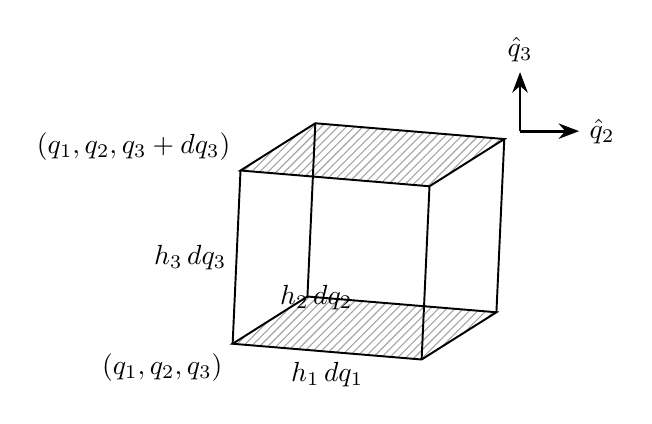
\begin{tikzpicture}[>={Stealth[length=2.6mm]}, line width=0.7pt]
  % vértices del paralelepípedo deformado (aristas no iguales)
  \coordinate (A) at (0,0);        % (q1,q2,q3)
  \coordinate (B) at (2.4,-0.2);   % + h1 dq1
  \coordinate (C) at (0.95,0.6);   % + h2 dq2
  \coordinate (D) at (0.1,2.2);    % + h3 dq3  -> (q1,q2,q3+dq3)
  \coordinate (BC) at (3.35,0.4);
  \coordinate (BD) at (2.5,2.0);
  \coordinate (CD) at (1.05,2.8);
  \coordinate (BCD) at (3.45,2.6);
  % caras q3 (inferior y superior) sombreadas
  \fill[pattern=north east lines, pattern color=black!35] (A)--(B)--(BC)--(C)--cycle;
  \fill[pattern=north east lines, pattern color=black!35] (D)--(BD)--(BCD)--(CD)--cycle;
  % aristas
  \draw (A)--(B)--(BC)--(C)--cycle;
  \draw (D)--(BD)--(BCD)--(CD)--cycle;
  \draw (A)--(D) (B)--(BD) (C)--(CD) (BC)--(BCD);
  % etiquetas de corner y aristas
  \node[below left] at (A){$(q_1,q_2,q_3)$};
  \node[above left] at (D){$(q_1,q_2,q_3+dq_3)$};
  \node[below] at ($(A)!0.5!(B)$){$h_1\,dq_1$};
  \node[above right] at ($(A)!0.5!(C)$){$h_2\,dq_2$};
  \node[left] at ($(A)!0.5!(D)$){$h_3\,dq_3$};
  % base curvilínea
  \draw[->, line width=1pt] (BCD)++(0.2,0.1)--($(BCD)+(0.95,0.1)$) node[right]{$\hat q_2$};
  \draw[->, line width=1pt] (BCD)++(0.2,0.1)--($(BCD)+(0.2,0.85)$) node[above]{$\hat q_3$};
\end{tikzpicture}
\end{document}
